%% \section{Background}
%% \label{sec:background}
%% \vs{background should be here. Needs background on Local and Gibbon.}
%% \mr{I introduced an Overview section that appears just before this one. Some of the material in the background section is now in Overview. Mostly the material is the high-level discussion. Now, the Background section will mainly be here to present the formalism, and anything not already introduced in the Overview.}

%% \note{new plan from Slack messages (VS): so really background could be why serializing helps (spatial locality == fast traversals)  + there is a compiler to automatically do this called gibbon + some local details?}
%% \mv{If this is just going to be an overview of the benefits of serialized heaps, is there a reason we can't just merge it into the previous section?}

%% In this section we present the Gibbon compiler in more detail, focusing in particular on its intermediate language and type system.
%% %
%% The Gibbon compiler uses LoCal~\cite{Local,gibbon-par} (\textbf{Lo}cation
%% \textbf{Cal}culus), a first-order intermediate representation (IR) where
%% programs are represented with an explicit byte-addressed, mostly-serialized data
%% layout. Gibbon translates programs into LoCal using \emph{location inference}, a
%% procedure built on top of region inference~\cite{regioncalcs} which annotates
%% programs with explicit location and region bindings and annotations. All values
%% reside within a region, which is (conceptually) an unbounded storage agea.
%% Locations are addresses within a region, and they are used for reading and
%% writing data. Locations roughly correspond to C's pointers but are less
%% flexible in that locations can only be written to once and arithmetic on
%% locations is highly restricted. A location is either: at the start of a region,
%% $N$ bytes past an existing location (to account for constant-sized data like integers), or \emph{after} the value at a particular
%% location (which may be constructed recursively). This serial ordering of locations is what ensures that the resulting
%% values are serialized in heap memory.
%% %
%% LoCal's type system tracks the data written to and read from
%% locations, ensuring that all data in all regions is well-typed.

%% \begin{figure}[]
%% \newcommand{\ctyatlocreg}[3]{\textcolor{emacsgreen}{#1}\textcolor{emacsbrown}{\bfseries\ensuremath{@}}\ensuremath{\locreg{#2}{#3}}}
%% \lstset{
%%     escapeinside={(@}{@)},          % if you want to add LaTeX within your code
%%     escapechar={\@},
%%     mathescape=true,
%% }
%% \begin{lstlisting}[ ]
%% 	data List = Cons Int List | Nil

%% 	@{\color{emacsblue}\text{mkList}}@ :: forall @\locreg{l}{r}@. Int -> @\ctyatlocreg{List}{l}{r}@
%% 	@{\color{emacsblue}\text{mkList}}@ [@\locreg{l}{r}@] n =
%% 	  if n == 0 then Nil @\locreg{l}{r}@ else
%% 	    @{\color{emacsblue}\texttt{letloc}}@ $\locreg{l_1}{r}$ = $\;\locreg{l}{r}$ + 9 in
%% 	    let tail: @\ctyatlocreg{List}{l_1}{r}@ = mkList [@\locreg{l_1}{r}@] (n-1) in
%% 	    Cons @\locreg{l}{r}@ n tail
%% \end{lstlisting}
%% \caption{\il{mkList} compiled into LoCal IR}\label{fig:mklist-LoCal}
%% \end{figure}

%% \begin{figure}[]
%% 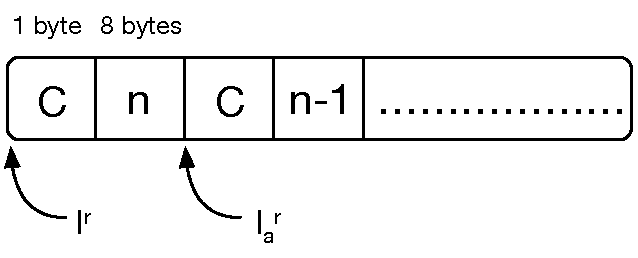
\includegraphics[scale=0.4]{figures/example1-list.pdf}
%% \caption{In-memory representation of list constructed by \il{mkList}}\label{fig:mklist-repr}
%% \end{figure}

%% An example LoCal program is shown in Figure~\ref{fig:mklist-LoCal}. The
%% \il{mkList} function takes a number \il{n} and a symbolic location \locreg{l}{r}
%% (read as: location \il{l} in region \il{r}), and returns a list of length \il{n}
%% at location \locreg{l}{r}. LoCal programs make use of a form of
%% \emph{destination-passing style}~\cite{destination-passing}, as the location
%% that the result will be written to is passed as an argument to the function.
%% %
%% If \il{n} is $0$, then \il{mkList} allocates \il{Nil} at location \locreg{l}{r}.
%% Otherwise, \il{mkList} must allocate a cons cell to \locreg{l}{r}. To do this, a
%% location $\locreg{l_1}{r}$ is introduced with a special \il{letloc} form, which
%% is 9 bytes past the location \locreg{l}{r} (one byte for the \il{Cons} tag and 8
%% bytes for the integer). Next, it recursively builds a list of length $(n-1)$ at
%% the newly bound location $\locreg{l_1}{r}$. Finally, it writes the \il{Cons} tag
%% and the integer \il{n}, completing the cons cell.
%% %
%% The resulting list is guaranteed by the types to be serialized in memory, within region \il{r}. Gibbon's location inference places all the cons cells in the same region because their allocations happen in order, ensuring the region will end up looking like the list in Figure~\ref{fig:mklist-repr}.

%% \mv{We can explain more about LoCal here if necessary. What do we need to establish about LoCal before moving on to section 4?}
